\subsection{Canal de comunicação}
% p01q01 - prova 2016/01
% ~/ee/ufsj/2016_01/ti/prova/prova01-resolucao.tex

\begin{questions}
\question{
Seja um canal de comunicação caracterizado por $p(y|x)$ dado abaixo

\begin{center}
\begin{tabular}{|c|c|c|}
\hline
\diagbox{X}{Y} & 0 & 1 \\
\hline
0 & 1/4 & 3/4 \\
\hline
1 & 2/3 & 1/3 \\
\hline
\end{tabular}
\end{center}
e uma fonte com distribuição dada por $p(x) = \left( 4/7, 3/7 \right)$.
% $p(y) = (3/7, 4/7)$

\begin{parts}
\part 
Calcule os valores das entropias $H(X)$ e $H(Y)$.

\part
Calcule a informação mútua $I(X;Y)$.

\part
Calcule as entropias condicionais $H(X|Y)$ e $H(Y|X)$, e também a entropia conjunta $H(X,Y)$.

\part
Seja $\widehat{X}$ um estimador para $X$ baseado em $Y$. Qual é o melhor estimador? 
Qual é a probabilidade de erro para este estimador? Compare com o limite imposto pela 
desigualdade de Fano.

\end{parts}
}

\begin{solution}
\begin{parts}
\part
  $H(X)$ pode ser calculado diretamente.

  \begin{eqnarray}
  H(X) &=& - \sum_{x \in \mathcal{X}} p(x) \log p(x) \\
        &=& - \frac{4}{7} \log \frac{4}{7} - \frac{3}{7} \log \frac{3}{7} \\
        &=&  \frac{4}{7} (\log 7 - \log 4) + \frac{3}{7} (\log 7 - \log 3) \\
        &=&  \log 7 - \frac{8}{7} - \frac{3}{7} \log 3 \\
        &=& 0.98523 \text{ bits}.
  \end{eqnarray}

  Para calcular os demais itens iremos precisar da distribuição conjunta 
  $p(x,y) = p(x) p(y|x) = p(y) p(x|y)$ dada por
  \begin{center}
  \begin{tabular}{|c|c|c|}
  \hline
  \diagbox{X}{Y} & 0 & 1 \\
  \hline
  0 & 1/7 & 3/7 \\
  \hline
  1 & 2/7 & 1/7 \\
  \hline
  \end{tabular}
  \end{center} 
  e também da marginal $p(y) = (3/7, 4/7)$. 

  Como a distribuição de $Y$ é apenas uma permutação da distribuição de $X$, teremos $H(Y) = H(X)$.

\part
  Utilizando a distribuição conjunta calculada no item anterior, temos
  \begin{eqnarray}
  I(X; Y) &=& \sum_{x, y} p(x,y) \log \frac{p(x,y)}{p(x)p(y)} \nonumber \\
        &=& \frac{1}{7} \log \left( \frac{1/7}{4/7 \times 3/7} \right) + \frac{3}{7} \log \left( \frac{3/7}{4/7 \times 4/7} \right)+ 
        \frac{2}{7} \log \left( \frac{2/7}{3/7 \times 3/7} \right) \nonumber \\
	&& + \frac{1}{7} \log \left( \frac{1/7}{3/7 \times 4/7} \right) \nonumber \\
        &=& \frac{1}{7} \log \left( \frac{7}{12} \right) + \frac{3}{7} \log \left( \frac{21}{16} \right) + \frac{2}{7} \log \left( \frac{14}{9} \right) + \frac{1}{7} \log \left( \frac{7}{12} \right) \nonumber \\
        &=& \log 7 \left( \frac{1}{7} + \frac{3}{7} + \frac{2}{7} + \frac{1}{7} \right) +
                \log 3 \left( -\frac{1}{7} + \frac{3}{7} - \frac{2}{7} \times 2 - \frac{1}{7} \right) \nonumber \\
	&& + \left( -\frac{1}{7} \times 2 - \frac{3}{7} \times 4 + \frac{2}{7} -\frac{1}{7} \times 2 \right) \nonumber \\
        &=& \log 7 - \frac{3}{7} \log 3 - 2 \nonumber \\
        &=& 0.12809\text{ bits}.
  \end{eqnarray}

\part
  \begin{eqnarray}
  H(X,Y) &=& H(X) + H(Y) - I(X;Y) \nonumber \\
        &=& 0.98523 + 0.98523 - 0.12809 = 1.8424 \nonumber \\ 
        &=& \log 7 - \frac{8}{7} - \frac{3}{7} \log 3 + \log 7 - \frac{8}{7} - \frac{3}{7} \log 3 - \left( \log 7 - \frac{3}{7} \log 3 - 2 \right) \nonumber \\
        &=& \log 7 - \frac{3}{7} \log 3 - \frac{2}{7} = 1.8424
  \end{eqnarray}

  \begin{eqnarray}
  H(Y|X) &=& H(X,Y) - H(X) = 0.85717 \\
        &=& \log 7 - \frac{3}{7} \log 3 - \frac{2}{7} - \left( \log 7 - \frac{8}{7} - \frac{3}{7} \log 3 \right) \\
        &=& \frac{6}{7}
  \end{eqnarray}

  \begin{equation}
  H(X|Y) = H(X,Y) - H(Y) = \frac{6}{7} = 0.85717
  \end{equation}


\part
  O melhor estimador é $\widehat{X} = 1 - Y$, ou seja,
  \begin{equation}
  \widehat{X} = \begin{cases} 
                0 & \mbox{ quando } Y = 1 , \\
                1 & \mbox{ quando } Y = 0 .
                \end{cases}
  \end{equation}

 
  A probabilidade de erro é dada por
  \begin{eqnarray}
  P_e &=& \textmd{Pr}\{\widehat{X}(Y) \neq X\} \nonumber \\
        &=& \textmd{Pr}\{Y = 0, X = 0\} + \textmd{Pr}\{Y = 1, X = 1\} \nonumber \\
        &=& 2 \times \frac{1}{7} = \frac{2}{7} 
  \end{eqnarray}

  A desigualdade de Fano estabelece que
  \begin{equation}
  H(P_e) + P_e \log \left( \vert \mathcal{X} \vert - 1 \right) \geq H(X|Y)
  \end{equation}
  Vamos utilizar a forma fraca da desigualdade de Fano, nos valendo de que $H(P_e) \leq 1$ e $\log \left( \vert \mathcal{X} \vert - 1 \right) \leq \log \left( \vert \mathcal{X} \vert \right)$.
  A forma fraca da desigualdade de Fano fornece o seguinte limite para a probabilidade de erro:
  \begin{equation}
  P_e \geq \frac{H(X|Y) - 1}{\log \left( \vert \mathcal{X} \vert \right)} = \frac{\frac{6}{7} - 1}{\log 2} = - \frac{1}{7} .
  \end{equation}
  %onde utilizamos que $H(P_e) \leq 1$ e $\log \left( \vert \mathcal{X} \vert - 1 \right) \leq \log \left( \vert \mathcal{X} \vert \right)$.
  A desigualdade encontrada não agrega informação, pois já sabemos previamente que $P_e \geq 0$. 
  Se analisarmos a desigualdade de Fano para o caso em que $\mathcal{X}$ é um alfabeto binário, teremos
  \begin{eqnarray}
  H(P_e) + P_e \log \left( \vert \mathcal{X} \vert - 1 \right) &\geq& H(X|Y) \nonumber \\
  H(P_e) + P_e \log \left( 2 - 1 \right) &\geq& H(X|Y) \nonumber \\
  H(P_e) &\geq& H(X|Y) \nonumber \\
  H(P_e) &\geq& \frac{6}{7}
  \end{eqnarray}
  Podemos ainda encontrar limites para $P_e$ analisando $H(P_e)$.

  \begin{lstlisting}[language=Octave]
Pe = [0.01:0.01:0.99];
HPe = -Pe.*log2(Pe) -(1-Pe).*log2(1-Pe);
id1 = find(HPe > 6/7, 1, 'first');
id2 = find(HPe > 6/7, 1, 'last');
figure; plot(Pe,HPe);
xlabel('Pe'); ylabel('H(Pe)');
line([Pe(id1) Pe(id1)],[0 HPe(id1)],'LineStyle','--');
line([Pe(id2) Pe(id2)],[0 HPe(id2)],'LineStyle','--');
line([0 Pe(id2)],[HPe(id1)  HPe(id1)],'LineStyle','--');
p1 = 0.001; H1 = 0;
while H1 < 6/7, p1=p1+0.001; H1=-p1.*log2(p1)-(1-p1).*log2(1-p1); end;
p2 = 0.6; H2 = 1;
while H2 > 6/7, p2=p2+0.001; H2=-p2.*log2(p2)-(1-p2).*log2(1-p2); end;
text(p1,-0.1,num2str(p1),'rotation',90);
text(p2,-0.1,num2str(p2),'rotation',90);
text(-0.05,6/7+0.01,'6/7');
axis([0 1 0 1]);
print -dsvg errorentropy.svg;
system('inkscape errorentropy.svg --export-pdf=errorentropy.pdf');
\end{lstlisting}

{\centering
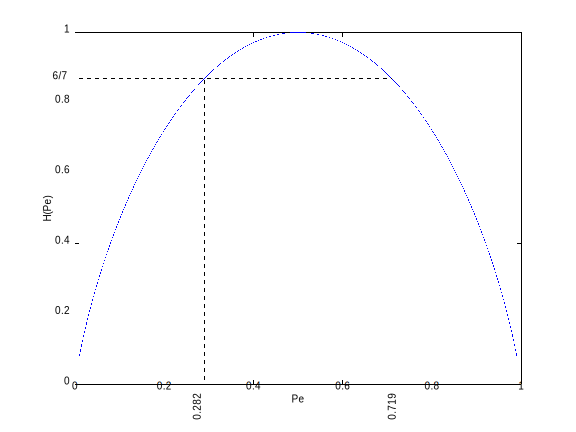
\includegraphics[width=0.5\textwidth]{../images/errorentropy.pdf}
}

Podemos observar então que $0.282 \leq P_e \leq 0.719$ satisfaz a condição $H(P_e) \geq 6/7$.
O valor exato de $P_e$ encontrado anteriormente, $P_e = 2/7 = 0.28571$ está neste intervalo.


\end{parts}
\end{solution}
\end{questions}
